\documentclass[letterpaper]{article}
\usepackage[margin=0.5 in, landscape]{geometry}
\pagestyle{empty}

% See https://pgfplots.sourceforge.net/gallery.html
% and https://tikz.dev/pgfplots/reference-3dplots

%\usepackage{capt-of}
\usepackage{fancyhdr}
\usepackage{lastpage}
\usepackage{caption}
\usepackage{amsmath}
\usepackage{esvect}
\usepackage{xcolor}
\usepackage{pgfplots}
\usepgfplotslibrary{patchplots}
\pgfplotsset{compat=newest}

% \usepackage[mode=buildnew]{standalone}
\usetikzlibrary{external}
\tikzexternalize[prefix=./tikz/]
 
% \title{Graphing Project}
% \author{Sean B}
% \date{September 2024}
\DeclareMathOperator{\proj}{proj}
\newcommand{\vct}{\mathbf}
\newcommand{\vctproj}[2][]{\proj_{\vct{#1}}\vct{#2}}

\pagestyle{fancy}
\renewcommand{\headrulewidth}{0pt}
\fancypagestyle{plain}{%
  \renewcommand{\headrulewidth}{0pt}%
  \fancyhf{}}

\fancyfoot[C]{\footnotesize{Sean Bradly, 2024}}%
\fancyfoot[R]{\footnotesize{\thepage\ of \pageref{LastPage}}}

\begin{document}
% \maketitle

% \section{Introduction}

\begin{figure}[!ht]
    \centering 
    \ \par\ \par\ \par\ \par\ \par\ \par\ \par\ \par\ \par
    \begin{tikzpicture}
        \begin{axis}[
            axis lines=center,
            view={25}{50},
            width={ 30 cm } ,
            height={ 24 cm},
            xlabel={$x$-axis},
            ylabel={$y$-axis},
            zlabel={$z$-axis},
            label style={color=black,font=\boldmath\Large},
            xmin=-10, xmax=10,
            ymin=-10, ymax=10,
            zmin=-10, zmax=10,
            xtick={-10,-5,5,10},ytick={-10,-5,5,10},ztick={-10,-5,5,10},
            minor tick={-10,-9,...,10},
        ]
            \addplot3[only marks,blue ] coordinates {(3, -4, -2)};
            \addplot3[blue!25, no marks, densely dashed] coordinates { (0, 0, -2) (3, 0, -2) (3,-4,-2) (0,-4,-2) (0, 0, -2)};
            \addplot3[blue!25, no marks, densely dashed] coordinates { (0, -4, -2) (0, -4, 0) (3,-4,0) (3,0,0) (3, 0, -2) };
            \addplot3[blue!25, no marks, densely dashed] coordinates { (3, -4, 0) (3, -4, -2) };
            \node [blue, below right] at (axis cs:3,-4,-2) {$A (3,-4,-2)$};
    
            \addplot3[only marks,olive  ] coordinates {(6,  5,  3)};
            \addplot3[olive!30, no marks, densely dashed] coordinates { (0, 0, 3) (6, 0, 3) (6,5,3) (0,5,3) (0, 0, 3)};
            \addplot3[olive!30, no marks, densely dashed] coordinates { (0, 5, 3) (0, 5, 0) (6,5,0) (6,0,0) (6, 0, 3) };
            \addplot3[olive!30, no marks, densely dashed] coordinates { (6, 5, 0) (6, 5, 3) };
            \node [olive, above right] at (axis cs:6,5,3) {$B (6,5,3)$};
    
            \addplot3[only marks,teal] coordinates {(4, -3,  6)};
            \addplot3[teal!35, no marks, densely dashed] coordinates { (0, 0, 6) (4, 0, 6) (4,-3,6) (0,-3,6) (0, 0, 6)};
            \addplot3[teal!35, no marks, densely dashed] coordinates { (0, -3, 6) (0, -3, 0) (4,-3,0) (4,0,0) (4, 0, 6) };
            \addplot3[teal!35, no marks, densely dashed] coordinates { (4, -3, 0) (4, -3, 6) };
            \node [teal, below left] at (axis cs:4,-3,6) {$C (4,-3,6)$};
    
        \end{axis}
    \end{tikzpicture}

    %\centering
    \caption{Plot of the Points $A(3,-4,-2)$, $B(6.5.3)$, and $C(4,-3,6)$}
\end{figure}

\pagebreak

\begin{figure}[!ht]
    \centering
    \ \par\ \par\ \par\ \par\ \par\ \par
    
    \begin{tikzpicture}
        \begin{axis}[
            axis lines=center,
            view={-165}{60},
            width={ 30 cm } ,
            height={ 24 cm},
            xlabel={$x$-axis},
            ylabel={$y$-axis},
            zlabel={$z$-axis},
            label style={color=black,font=\boldmath\Large},
            xmin=-1, xmax=5,
            ymin=-5, ymax=1,
            zmin=-2, zmax=2,
            xtick={-1,...,5},ytick={-5,...,1},ztick={-2,...,2},
            minor tick={-2,-1,0,1,2},
        ]
            \addplot3[blue, ->] coordinates { (0, 0, 0) (2, -4, 1) };
            \addplot3[blue!20, no marks, densely dashed] coordinates { (0, 0, 1) (2, 0, 1) (2,-4,1) (0,-4,1) (0, 0, 1)};
            \addplot3[blue!20, no marks, densely dashed] coordinates { (0, -4, 1) (0, -4, 0) (2,-4,0) (2,0,0) (2, 0, 1) };
            \addplot3[blue!20, no marks, densely dashed] coordinates { (2, -4, 0) (2, -4, 1) };
            \node [blue, above right] at (axis cs:2,-4,1) {$\vv{u} = \langle 2,-4,1 \rangle$};
    
            \addplot3[teal, ->] coordinates { (0, 0, 0) (3, 0, -1) };
            \addplot3[teal!30, no marks, densely dashed] coordinates { (0, 0, -1) (3, 0, -1) };
            \addplot3[teal!30, no marks, densely dashed] coordinates { (3, 0, 0) (3, 0, -1) };
            \node [teal, below left] at (axis cs:3,0,-1) {$\vv{v} = \langle 3,0,-1 \rangle$};
    
        \end{axis}
    \end{tikzpicture}
    \caption{ Plot vectors: $\protect\vv{u} = \langle 2,-4,1 \rangle$ to $\protect\vv{v} = \langle 3,0,-1 \rangle$ }
\end{figure}

\pagebreak

\begin{figure}[!ht]
    \ \par\ \par\ \par\ \par
    \centering
    \begin{tikzpicture}
        \begin{axis}[
            axis lines=center,
            view={-135}{30},
            width={ 30 cm } ,
            height={ 24 cm},
            xlabel={$x$-axis},
            ylabel={$y$-axis},
            zlabel={$z$-axis},
            label style={color=black,font=\boldmath\Large},
            xmin=-1, xmax=5,
            ymin=-5, ymax=1,
            zmin=-1, zmax=2,
            ticks = none,
            % xtick={-1,...,5},ytick={-5,...,1},ztick={-2,...,2},
            % minor tick={-2,-1,0,1,2},
        ]
            \addplot3[blue, ->] coordinates { (0, 0, 0) (2, -4, 1) };
            \addplot3[blue!30, no marks, dashed] coordinates { (3, 0, -1) (5, -4, 0) };
            % \addplot3[blue, no marks, densely dashed] coordinates { (0, 0, 1) (2, 0, 1) (2,-4,1) (0,-4,1) (0, 0, 1)};
            % \addplot3[blue, no marks, densely dashed] coordinates { (0, -4, 1) (0, -4, 0) (2,-4,0) (2,0,0) (2, 0, 1) };
            % \addplot3[blue, no marks, densely dashed] coordinates { (2, -4, 0) (2, -4, 1) };
            \node [blue, above right] at (axis cs:2,-4,1) {$\vv{u} = \langle 2,-4,1 \rangle$};
    
            \addplot3[teal, ->] coordinates { (0, 0, 0) (3, 0, -1) };
            \addplot3[teal!35, no marks, dashed] coordinates { (2, -4, 1) (5, -4, 0) };
            % \addplot3[teal, no marks, densely dashed] coordinates { (0, 0, -1) (3, 0, -1) };
            % \addplot3[teal, no marks, densely dashed] coordinates { (3, 0, 0) (3, 0, -1) };
            \node [teal, below left] at (axis cs:3,0,-1) {$\vv{v} = \langle 3,0,-1 \rangle$};
    
            \addplot3[magenta, ->] coordinates { (0, 0, 0) (5, -4, 0) };
            \addplot3[magenta!30, no marks, densely dashed] coordinates { (5, 0, 0) (5, -4, 0) };
            \addplot3[magenta!30, no marks, densely dashed] coordinates { (0, -4, 0) (5, -4, 0) };
            \node [magenta, above left] at (axis cs:5,-4,0) {$\vv{u}+\vv{v} = \langle 5,-4,0 \rangle$};
    
        \end{axis}
    \end{tikzpicture}
    
    \caption{ Plot $ \protect\vv{u} + \protect\vv{v} $ from Figure 2 }
\end{figure}

\pagebreak

\begin{figure}[!ht]

    \ \par\ \par\ \par\ \par\ \par
    \centering

    \begin{tikzpicture}
        \begin{axis}[
            axis lines=center,
            view={-135}{30},
            width={ 15 cm } ,
            height={ 15 cm},
            xlabel={$x$},
            ylabel={$y$},
            label style={color=black,font=\boldmath\Large},
            xmin=0, xmax=6,
            ymin=0, ymax=6,
            xtick={0,...,5},ytick={0,...,5},
            minor tick={-2,-1,0,1,2},
            axis equal,
            grid=both
        ]
            % u
            \addplot[blue,  ->] coordinates { (0,0) (3,2)  };
            \addplot[blue, no marks] coordinates { (0,0) (3,2)  };
            \node [blue, above right] at (axis cs:3,2) {$\vv{u}=\langle 3,2\rangle$};
    
            % v
            \addplot[cyan,->] coordinates { (0,0) (2,5) };
            \addplot[cyan, no marks, dashed] coordinates { (0,0) (2,5) };
            \node [cyan, above right] at (axis cs:2,5) {$\vv{v}=\langle 2,5\rangle$};
    
            % proj_v u =  <32/29, 80/29> =~ <1.1034, 2.7586>
            \addplot[red, -> ] coordinates { (0,0) (1.1034,2.7586) };
            \addplot[red, no marks, dashed] coordinates { (0,0) (1.1034,2.7586) };
            \node [red, above right] at (axis cs:1.3034,2.7586) {$\vctproj[v]{u}=\langle \frac{32}{29},\frac{80}{29} \rangle$};
    
            % 
            \addplot[black, no marks, densely dashed] coordinates { (3,2) (1.1034,2.7586) };
            \addplot[black, no marks] coordinates { (1.0292,2.5729)  (1.21486547876830, 2.49864721620730) (1.28914361403912, 2.68434255438435) };
            % \draw [black, thick,dashed] (axis cs:0.5,0) arc [start angle=33.69,end angle=68.20,radius=0.5];
            \draw [black, domain=33.69:68.20] (axis cs:0,0) plot ({cos(\x) * 0.5}, {sin(\x) * 0.5});
            \node [black, above right] at (axis cs:0.405,0.04) {$\cos \theta = \frac{u \cdot v}{\left|u\right| \left|v\right|}$};
    
            % redraw v for dashes
            % \addplot[cyan, no marks, dashed] coordinates { (0,0) (2,5) };
    
    
        \end{axis}
    \end{tikzpicture}

    \caption{Plot $\protect\vv{u} = \langle 3,2 \rangle$ and $ \protect\vv{v} = \langle 2,5 \rangle $ and $\protect\vctproj[v]{u}$ }
\end{figure}

\pagebreak

\begin{figure}[!ht]

    \ \par\ \par\ \par\ \par\ \par
    \centering 
    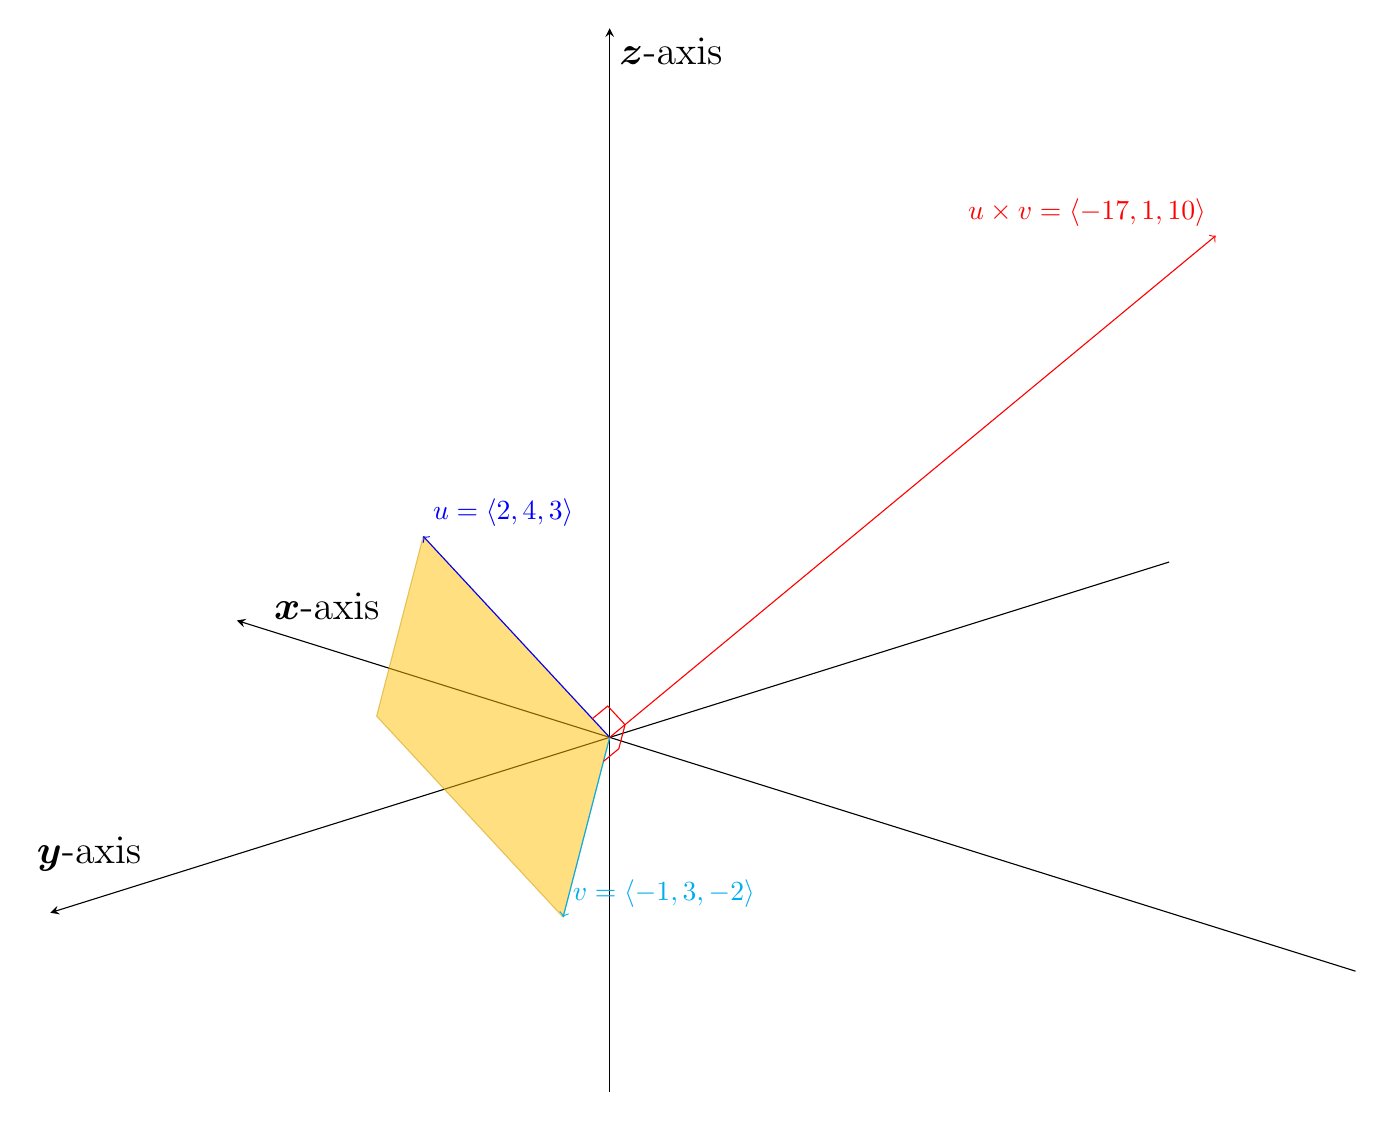
\begin{tikzpicture}
        \begin{axis}[
            axis lines=center,
            view={225}{25},
            width={ 30 cm } ,
            height={ 24 cm},
            xlabel={$x$-axis},
            ylabel={$y$-axis},
            zlabel={$z$-axis},
            label style={color=black,font=\boldmath\Large},
            xmin=-20, xmax=10,
            ymin=-20, ymax=20,
            zmin=-5, zmax=10,
            ticks=none,
        ]

            % u = vector([2,4,3])
            % v = vector([-1,3,-2])
            % uxp = u.cross_product(v)
            
            % print(u)
            % print("uxp: {}, normalized: {}".format(uxp, uxp.normalized().n()))
            % u+v
            
            % ut = u.normalized().n() * 0.5 
            % uxt = uxp.normalized().n()*0.5
            % print((ut, ut + uxt, uxt))
            
            % vt = v.normalized().n() * 0.5 
            % vxt = uxp.normalized().n()*0.5
            % print((vt, vt + vxt, vxt))
                        
            % |u x v| -- y u no black?!?
            \addplot3[opacity=0.5, color = black, fill = black, patch, patch type=polygon, vertex count=4] coordinates {
                (0,0,0)
                (2,4,3)
                (1,7,1)
                (-1,3,-2)
            };
    
            % u
            \addplot3[blue, ->] coordinates { (0, 0, 0) (2, 4, 3) };
            \node [blue, above right] at (axis cs:2,4,3) {$\vv{u} = \langle 2,4,3 \rangle$};
    
            % v
            \addplot3[cyan, ->] coordinates { (0, 0, 0) (-1, 3, -2) };
            \node [cyan, above right] at (axis cs:-1,3,-2) {$\vv{v} = \langle -1,3,-2 \rangle$};
    
            % u x v
            \addplot3[red, ->] coordinates { (0, 0, 0) (-17, 1, 10) };
            \node [red, above left] at (axis cs:-17,1,10) {$\vv{u} \times \vv{v} = \langle -17,1,10 \rangle $};
    
            % u & uxv right angle mark
            \addplot3[red, no marks] coordinates { 
                (0.185695338177052, 0.371390676354104, 0.278543007265578)
                (-0.244718892833506, 0.396709160531195, 0.531727849036494)
                (-0.430414231010558, 0.0253184841770917, 0.253184841770917)
            };        
            % v & uxv right angle mark
            \addplot3[red, no marks] coordinates { 
                (-0.133630620956212, 0.400891862868637, -0.267261241912424)
                (-0.564044851966770, 0.426210347045728, -0.0140764001415077)
                (-0.430414231010558, 0.0253184841770917, 0.253184841770917)
            };
    
        \end{axis}
    \end{tikzpicture}
    
    \caption{Plot $\protect\vv{u} \times \protect\vv{v}$ where $\protect\vv{u} = \langle 2,4,3 \rangle $ and $\protect\vv{u} = \langle -1,3,-2 \rangle $ }
\end{figure}


\pagebreak

\begin{figure}[!ht]

    \ \par\ \par\ \par\ \par\ \par\ \par
    \centering 
    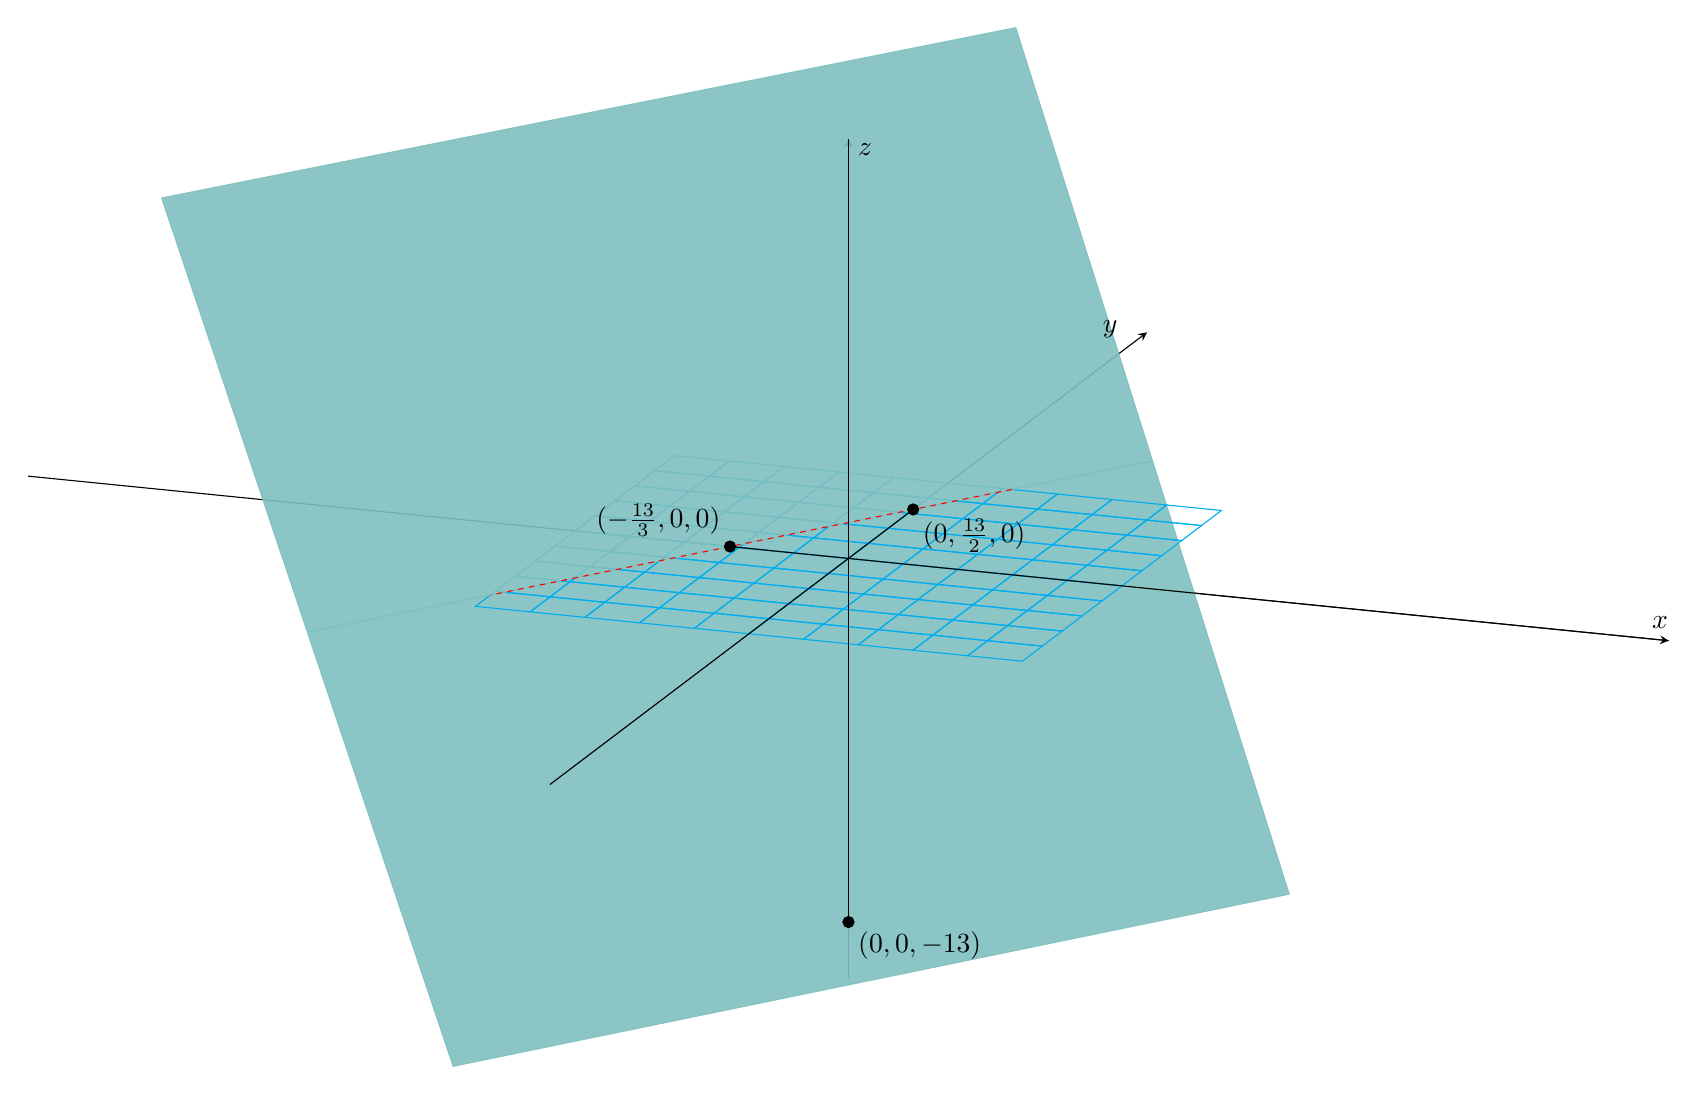
\begin{tikzpicture}
        \begin{axis}[
            axis lines=center,
            view={20}{16},
            width={ 30 cm } ,
            height={ 24 cm},
            xlabel={$x$},
            ylabel={$y$},
            zlabel={$z$},
            % label style={color=black,font=\boldmath\Large},
            xmin=-30, xmax=30,
            ymin=-30, ymax=30,
            zmin=-15, zmax=15,
            unit vector ratio=1 1 1,
            % 3d box=complete
            xtick=\empty,
            ytick=\empty,
            ztick=\empty,
        ]

            % plane < x-y
            \addplot3[
                patch,
                patch type=rectangle,
                color=teal!50,
                faceted color=none,
                opacity=0.9
            ] table[row sep=crcr, point meta=\thisrow{c}] { %
                x      y   z   c \\
                -14.33 -15 0   0 \\
                -9     -15 -15 0 \\
                10.66  15  -15 0 \\
                5.66   15  0   0 \\
            };

            % x-y grid
            \addplot3[mesh, cyan, thin, domain=-10:10, samples=11, domain y=-10:10, samples y=11, forget plot] {0};

            % plane > x-y            
            \addplot3[
                patch,
                patch type=rectangle,
                color=teal!50,
                faceted color=none,
                opacity=0.9
            ] table[row sep=crcr, point meta=\thisrow{c}] { %
                x      y   z  c \\
                5.66   15  0  0 \\
                -14.33 -15 0  0 \\
                -19.66 -15 15 0 \\
                0.66   15  15 0 \\
            };

            % intersection
            \addplot3 [red, dash pattern=on 2pt off 2pt ] coordinates { (7/3, 10 , 0)  (-10, -17/2, 0) };
            
            % redraw axis
            \addplot3 [black] coordinates { (-13/3, 0 , 0)  (30, 0, 0) };
            \addplot3 [black] coordinates { (0, 13/2 , 0)  (0, -30, 0) };
            \addplot3 [black] coordinates { (0, 0 , -13)  (0, 0, 15) };

            % points / labels
            \addplot3 [black, only marks] coordinates { (0, 0 , -13)  (-13/3, 0 , 0)  (0, 13/2, 0) };
            \node [black, below right] at (axis cs:0,0,-13) {$(0,0,-13)$};
            \node [black, above left] at (axis cs:-4.33,0,0) {$(-\frac{13}{3},0,0)$};
            \node [black, below right] at (axis cs:0,6.5,0) {$(0,\frac{13}{2},0)$};

        \end{axis}
    \end{tikzpicture}
    
    \caption{Graph the plane: $3x - 2y+z=-13$}
\end{figure}

\pagebreak

\begin{figure}[!ht]

    \ \par\ \par\ \par\ \par\ \par\ \par\ \par\ \par
    \centering 
    \begin{tikzpicture}
        \begin{axis}[
            axis lines=center,
            view={39}{56},
            width={ 30 cm } ,
            height={ 24 cm},
            xlabel={$x$},
            ylabel={$y$},
            zlabel={$z$},
            % label style={color=black,font=\boldmath\Large},
            xmin=-8, xmax=8,
            ymin=-8, ymax=8,
            zmin=-8, zmax=8,
            % 3d box=complete
            xtick=\empty,
            ytick=\empty,
            ztick=\empty,
        ]

        % bottom
        \addplot3[surf, colormap/viridis, opacity=0.35, samples=150, 
            y filter/.expression={ (y<0) ? ( (x<=0) ? y : -inf) : y },
            restrict expr to domain={((x^2/4)+(y^2/9)-1>=0)*(y>=0)}{-5:5}
        ] 
        {
            -sqrt((x^2/4)+(y^2/9)-1)
        };

        \addplot3[surf, colormap/viridis, opacity=0.35, samples=150, opacity=0.05,
            y filter/.expression={ (y<0) ? ( (x<=0) ? -inf : y ) : -inf },
            restrict expr to domain={((x^2/4)+(y^2/9)-1>=0)*(y>=0)}{-5:5}
        ] 
        {
            -sqrt((x^2/4)+(y^2/9)-1)
        };

        % top
        \addplot3[surf,colormap/viridis, opacity=0.35, samples=150,
            y filter/.expression={ (y<0) ? ( (x<=0) ? y : -inf) : y },
            restrict expr to domain={((x^2/4)+(y^2/9)-1>=0)*(y>=0)}{-5:5}
        ] 
        {
            sqrt((x^2/4)+(y^2/9)-1)
        };

        \addplot3[surf, colormap/viridis, opacity=0.35, samples=150, opacity=0.05,
        y filter/.expression={ (y<0) ? ( (x<=0) ? -inf : y ) : -inf },
        restrict expr to domain={((x^2/4)+(y^2/9)-1>=0)*(y>=0)}{-5:5}
        ] 
        {
            sqrt((x^2/4)+(y^2/9)-1)
        };


        \addplot3[opacity=0.2, color = black, fill = black, patch, patch type=polygon, vertex count=4] coordinates {
            (2-0.25, 0, 2.29+0.25)
            (5+0.25, 0, 2.29+0.25)
            (5+0.25, 0, -2.29-0.25)
            (2-0.25, 0, -2.29-0.25)
        };

        \addplot3[opacity=0.2, color = black, fill = black, patch, patch type=polygon, vertex count=4] coordinates {
            (0, -3+0.25, 1.33+0.25)
            (0, -5-0.25, 1.33+0.25)
            (0, -5-0.25, -1.33-0.25)
            (0, -3+0.25, -1.33-0.25)
        };

        \addplot3 [ultra thick,black,domain=2:5,samples=50,samples y=1] ( {x}, {0}, {sqrt((x^2/4)-1)} );
        \addplot3 [ultra thick,black,domain=2:5,samples=50,samples y=1] ( {x}, {0}, {-sqrt((x^2/4)-1)} );
        \addplot3 [ultra thick,black,domain=3:5,samples=50,samples y=1] ( {0}, {-x}, {sqrt((x^2/9)-1)} );
        \addplot3 [ultra thick,black,domain=3:5,samples=50,samples y=1] ( {0}, {-x}, {-sqrt((x^2/9)-1)} );

        % \addplot3 [black, ->] coordinates { (-0.25,0,0) (1.75,0,0) };
        % \addplot3 [black, ->] coordinates { (0,0.25,0) (0,-2.75,0) };
        % \addplot3 [black, ->] coordinates { (0,0,-0.75) (0,0,3) };
        

        \addplot3 [ultra thick,black,domain=3:5,samples=50,samples y=1] ( {0}, {-x}, {-sqrt((x^2/9)-1)} );

        % \node [black, below left] at (axis cs:0,-5,-5) {Note: surface is symmetric about the $xz$ plane. $y<0$ omitted to show detail.};

        \end{axis}
    \end{tikzpicture}
    
    \caption{Graph $\frac{x^2}{4} + \frac{y^2}{9} - z^2 = 1$}
\end{figure}

\pagebreak

\begin{figure}[!ht]

    \ \par\ \par\ \par\ \par\ \par\ \par
    \centering 
    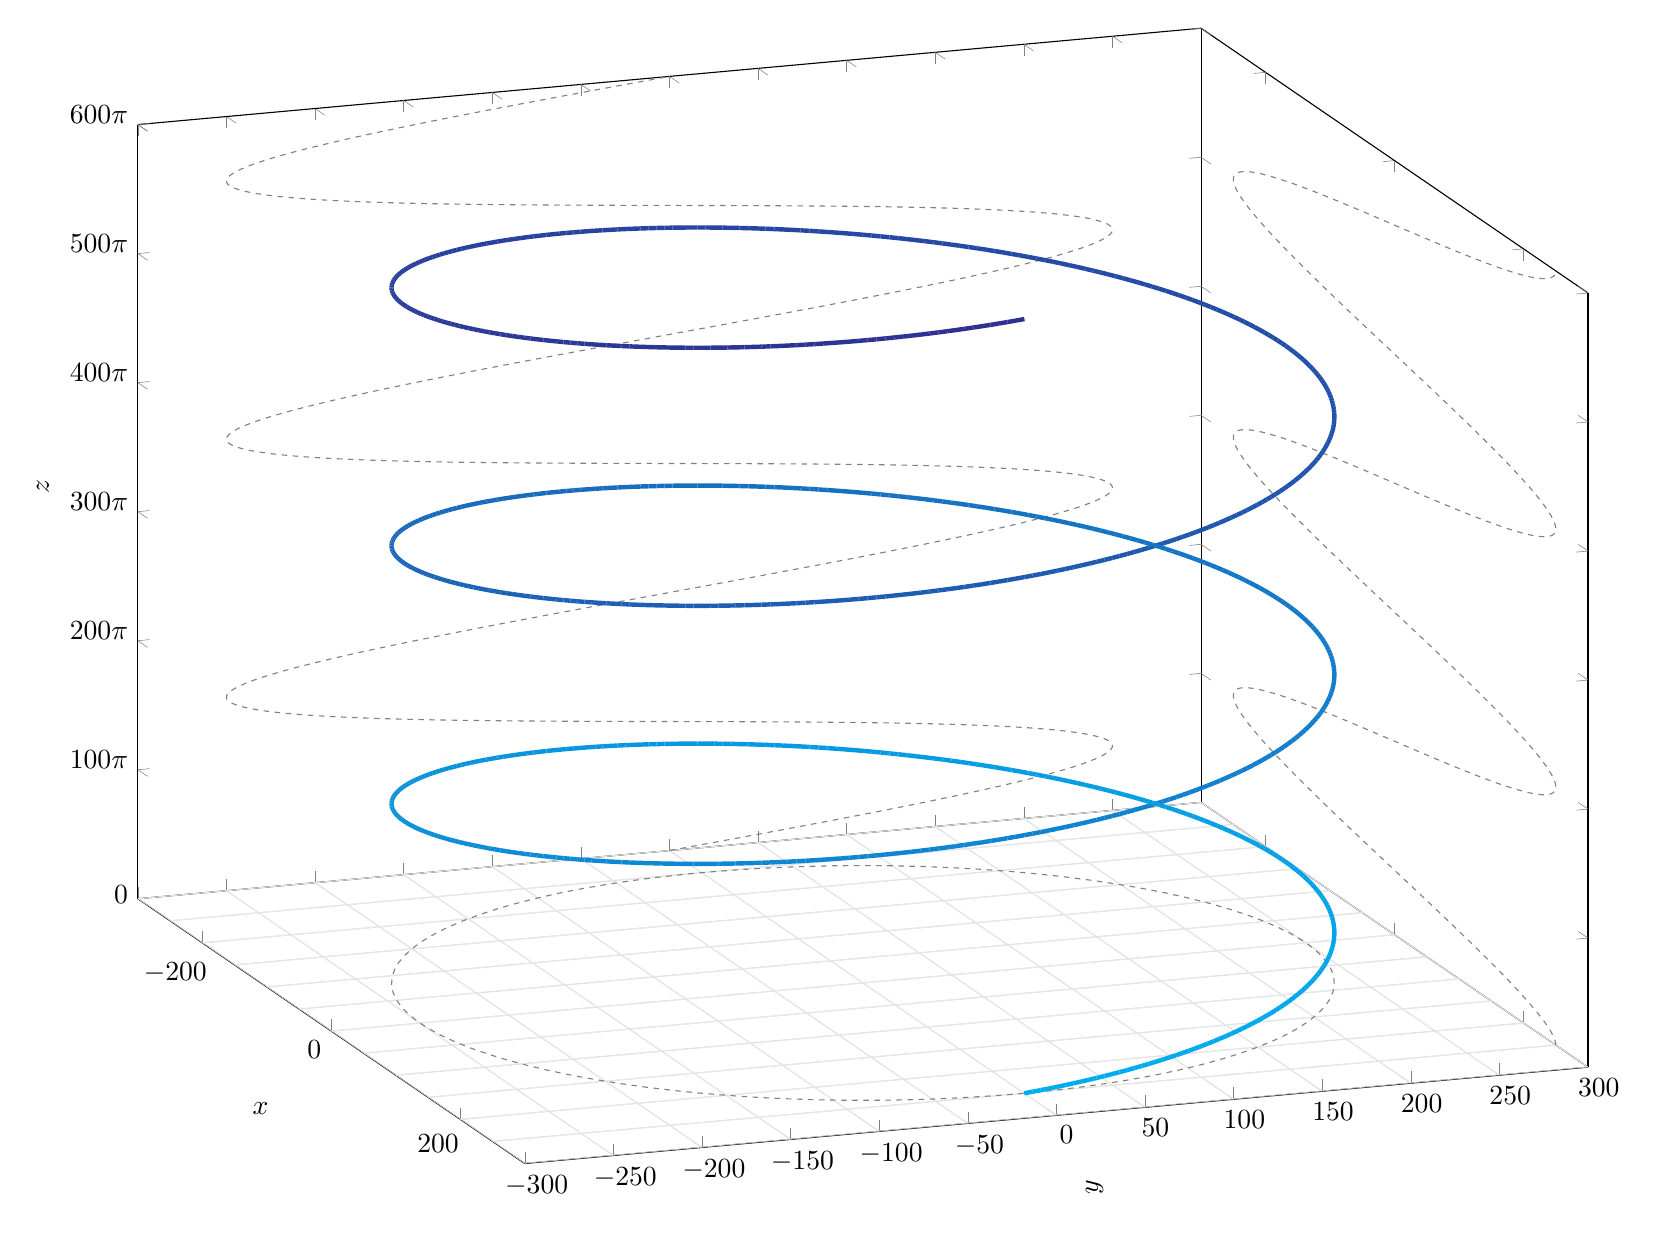
\begin{tikzpicture}
        \begin{axis}[
            axis lines=box,
            view={70}{20},
            width={ 20 cm } ,
            height={ 16 cm},
            xlabel={$x$},
            ylabel={$y$},
            zlabel={$z$},
            % label style={color=black,font=\boldmath\Large},
            xmin=-300, xmax=300,
            ymin=-300, ymax=300,
            zmin=0, zmax=6*pi*100,
            ztick={0, 3.14159*100, 3.14159*2*100, 3.14159*3*100, 3.14159*4*100, 3.14159*5*100, 3.14159*6*100},
            zticklabels={$0$, $100\pi$, $200\pi$, $300\pi$, $400\pi$, $500\pi$, $600\pi$},
            % 3d box=complete
            % xtick=\empty,
            % ytick=\empty,
            % ztick=\empty,
        ]

        \addplot3[mesh, gray!20, domain=-300:300, samples=13, domain y=-300:300, samples y=13, forget plot] {0};

        \addplot3 [black!50, thin, domain=0:2*pi, samples=100, samples y=1, dash pattern=on 2pt off 2pt] ( {250*cos(deg(x))}, {250*sin(deg(x))}, {0});
        \addplot3 [black!50, thin, domain=0:6*pi, samples=600, samples y=1, dash pattern=on 2pt off 2pt] ( {-300}, {250*sin(deg(x))}, {100*x});
        \addplot3 [black!50, thin, domain=0:6*pi, samples=600, samples y=1, dash pattern=on 2pt off 2pt] ( {250*cos(deg(x))}, {300}, {100*x});

        \addplot3 [black, ultra thick, domain=0:6*pi, samples=1000, samples y=1,
        mesh, % Use line segments instead of one unbroken line
        colormap={}{ % Define the colormap
            color(0cm)=(cyan);
            color(1cm)=(blue);
        },
        ] ( {250 * cos(deg(x))}, { 250 * sin(deg(x)) }, {100*x} );

        \end{axis}
    \end{tikzpicture}
    
    \caption{Graph $ \langle 250\cos t, 250 \sin t, 100t \rangle $}
\end{figure}

\pagebreak

\begin{figure}[!ht]

    \centering
    \ \par\ \par
    
    \begin{tikzpicture}
        \begin{axis}[
            axis lines=box,
            view={165}{60},
            width={ 22 cm } ,
            height={ 18 cm},
            xlabel={$x$},
            ylabel={$y$},
            zlabel={$z$},
            % label style={color=black,font=\boldmath\Large},
            xmin=-2, xmax=2,
            ymin=-2, ymax=2,
            zmin=-2, zmax=2,
            % 3d box=complete
            xtick={-2,-1,0,1,2},
            ytick={-2,-1,0,1,2},
            ztick={-2,2},
        ]

        \addplot3[mesh, gray!20, domain=-2:2, samples=11, domain y=-2:2, samples y=11, forget plot] {-2};


        \addplot3[surf, colormap/jet, opacity=0.45, samples=100, domain=-2:2] 
        {
            (4*x*y) / (3*x^2 + y^2)
        };

        % \node [black, below left] at (axis cs:0,-5,-5) {Note: surface is symmetric about the $xz$ plane. $y<0$ omitted to show detail.};

        \end{axis}
    \end{tikzpicture}
    
    \caption{Graph $z = \frac{4xy}{3x^2 + y^2}$}
\end{figure}

\end{document}
